\section{Auswertung}
\label{sec:Auswertung}

\subsection{Statistik des alpha-Zerfalls}

m:  533.9755
bins:  [ 495.8  505.2  514.6  524.   533.4  542.8  552.2  561.6  571.   580.4
  589.8]
n:  [  9.  24.  28.  40.  38.  26.  19.  13.   2.   1.]
halo i bims, 1 echter balken:  [500 509 519 528 538 547 556 566 575 585]
halo i bims, 1 gauß:  [ 19.81087747] +/- [ 1.07412195]


Die genommenen Messwerte wurden als normiertes Histogram in Abb. \ref{fig:hist} dargestellt, d.h. das Histogram wurde so normiert, dass die Summe über alle Balken 1 beträgt. Die eingezeichnete Fit-Kurve stellt eine Gauß-Normalverteilung gemäß
\begin{equation}
  G(x) = \frac{A}{\sigma\cdot\sqrt(2\pi)}e^{-0.5 {\frac{x-m}{\sigma}}^2}
  \label{eqn:gauß}
\end{equation}
dar. Hierbei ist  $\sigma=19.81 \pm 1.07$ die Standardabweichung und $m= 533.98$ der Mittelwert der aufgenommenen Werte.

 \begin{figure}
   \centering
   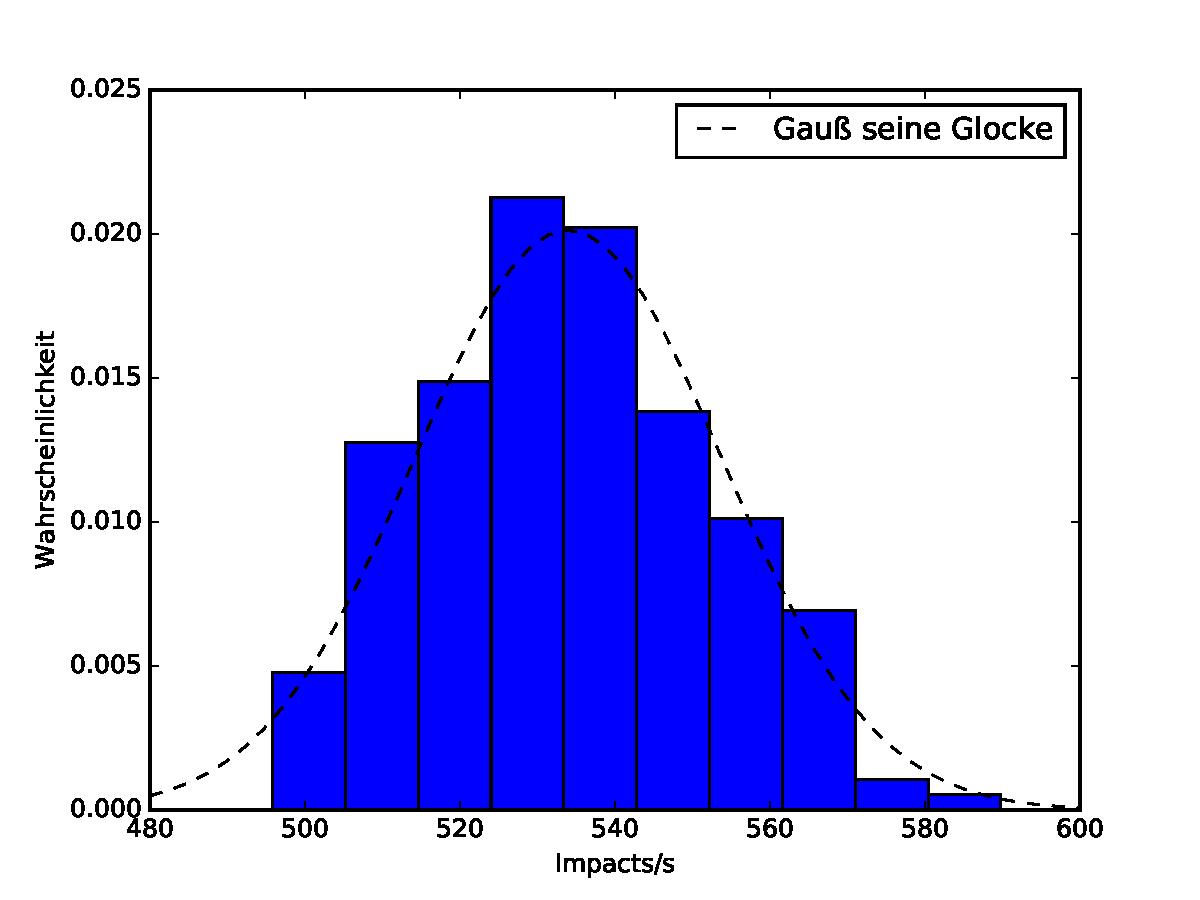
\includegraphics[height=6cm]{plots/Statistik.pdf}
   \caption{Histogram zur Zählrate}
   \label{fig:hist}
 \end{figure}
